%!TEX TS-program = /opt/local/bin/pdflatex
% TEMPLATE for Usenix papers, specifically to meet requirements of
%  USENIX '05
% originally a template for producing IEEE-format articles using LaTeX.
%   written by Matthew Ward, CS Department, Worcester Polytechnic Institute.
% adapted by David Beazley for his excellent SWIG paper in Proceedings,
%   Tcl 96
% turned into a smartass generic template by De Clarke, with thanks to
%   both the above pioneers
% use at your own risk.  Complaints to /dev/null.
% make it two column with no page numbering, default is 10 point

% Munged by Fred Douglis <douglis@research.att.com> 10/97 to separate
% the .sty file from the LaTeX source template, so that people can
% more easily include the .sty file into an existing document.  Also
% changed to more closely follow the style guidelines as represented
% by the Word sample file. 
% This version uses the latex2e styles, not the very ancient 2.09 stuff.
\documentclass[letterpaper,twocolumn,10pt]{article}
\usepackage{usenix,epsfig,endnotes,graphicx}
\begin{document}

%don't want date printed
\date{}

%make title bold and 14 pt font (Latex default is non-bold, 16 pt)
\title{\Large \bf Intellidrive: Improving Disk Drive Read Access with Machine \\ Learning Algorithms}

\author{
{\rm Peter Gebhard}\\
\and
{\rm Philip Joseph}\\
University of Illinois at Urbana-Champaign \\
Department of Computer Science
\and
{\rm Vance Thornton}\\
} % end author

\maketitle

% Use the following at camera-ready time to suppress page numbers.
% Comment it out when you first submit the paper for review.
\thispagestyle{empty}

\section{Introduction}

In the unwavering demand for ever faster computing, we have grown accustomed to a relatively stagnant rate of improvement in hard disk drive access times ~\cite{CachingStrategies}.  Meanwhile, advances in CPU, GPU, and RAM technologies continue to push the limits of performance.  It is from these observations that we are focusing on a method to alleviate the disk drive from its mechanical limitations and improve it's perceived performance through more sophisticated caching.

The typical approach to solving data latency issues is to build a caching store as a new layer between the requester and the requestee.  To improve disk drive access performance, modern hard disk drives now commonly include a read/write disk buffer that allows the disk drive to cache sectors ahead of (and possibly behind) a requested sector read ~\cite{MultiplePrefetch}.  This same disk buffer can also be used to queue incoming write requests so the system's OS can continue other processing.  So while most system disks already contain a disk buffer, we feel that disk read performance can be improved by moving beyond a simplistic read-ahead approach and instead applying a machine learning algorithm.  Our approach will not focus on any significant changes to how write requests are queued and scheduled.

In current approaches much of the responsibility for data access performance is placed on the application developer.  Decisions regarding the use of files and the organization of data within files can have a significant impact on data access performance.  Choosing an appropriate data organization can be a difficult task that is even more difficult when it is not known in advance what the common access patterns will be.  Current approaches attempt to ease this burden by providing caching based on simple assumptions such as that data that was accessed recently is more likely to be accessed again soon and that data that is near data that is being read in a file is likely to be read soon.  Existing file system implementations attempt to reorganize data so that files are stored sequentially on the disk.  Whether or not these assumptions about disk access patterns and appropriate block organization are correct is highly application dependent and may change over time.

Our approach has the potential to be better than current approaches because the access pattern prediction utilizes more sophisticated models that are based on access history and adapt over time.  By providing dynamic block reorganization we will also hopefully reduce or eliminate the need for application developers to consider the performance implications of data organization as data organization will adapt over time based on usage.

The anticipated result of this project is that disk read performance will be improved for tasks that require repeated random I/O for sets of related data.  Improving write performance is not a goal of this project, however a potential benefit of intelligent block reorganization is that random writes can be replaced with sequential writes which are later reorganized based on access patterns.

\section{Design}
\subsection{System Architecture}
The Intellidrive system is composed two main components, a block device driver and a daemon for servicing requests from the block device driver.  The user file system makes use of the block device driver to store information.  The block device driver forwards the requests to a user space daemon which processes the requests.  In order to achieve high performance as well as insure contiguous block storage and avoid unnecessary additional caching the daemon stores and retrieves blocks using a raw partition.  An overview of the Intellidrive system architecture is shown in the diagram below:

\begin{figure*}[htb]
  \center{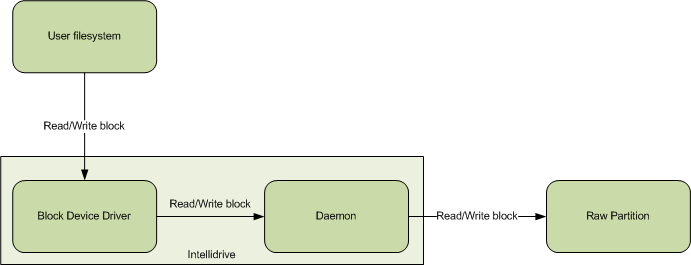
\includegraphics[width=\textwidth]
  {system-architecture.png}}
  \caption{Intellidrive System Architecture}
\end{figure*}

The philosophy behind this design is that the block device driver should be as simple as possible.  The daemon is responsible for most of the functionality of the system.  In addition to servicing block read/write requests the daemon also performs device access logging, block precaching, and periodic drive optimization.

\subsection{Block Device Driver}

In our preliminary design discussions, it was thought that block device driver would contain all the functionality of the Intellidrive system.  In that role, the block device driver would handle all incoming read and write requests by processing them and updating its internal data structures representing the logical block map and block access log.  Beyond recording this metadata, the block device driver would act like any other device driver that abstracts a hard disk and it would transparently ensure that all read and write requests were fulfilled.

As our research continued, it became clear that there were still more issues to consider.  First, it would not be a simple task to maintain the mappings and logs in files on the disk because the block device driver was already operating at a level below the existing file system.  It appeared that we would be limited to maintaining our data structures within main memory and being forced to incur the overhead that  was introduced.  Second, it was difficult to consider how any block rearrangement could be performed seamlessly since it seemed that it may be necessary to unmount a drive to perform the rearrangement.  In the long run, this would not be an adequate solution. 

It was decided that a user-space daemon would make it possible to easily store our logs and mappings as files on the disk.  Additionally, the daemon would include the algorithm used for block rearrangement.  Through our logical to physical block mapping, which acts as an indirection table, we are able to interpret an incoming block request and have it access a different physical block on the drive.  At the same time, this block mapping allows the daemon to perform rearrangements on the disk in the background, so long as all rearranged physical blocks have their value in the mapping updated to match the new arrangement.

\subsection{Logical to Physical Block Mapping}

In order to support intelligent block reorganization Intellidrive maps logical block numbers to physical block numbers.  This is implemented using an array where the value stored at element N is the physical block number of logical block number N.  If 4KB blocks are used this map requires 1 megabyte of memory for every gigabyte of drive storage capacity.

\subsection{Precache Boundaries}

Intellidrive makes use of precache groups to represent groups of blocks that should be precached together.  During drive idle time blocks sequentially following recently read blocks are precached into memory until a precache boundary is reached.  The precache boundaries are represented using a bit vector where the bit stored at position M in the vector has a value of 1 if precaching should stop after block number M has been precached.  Represented as a bit vector the precache boundaries require 32KB of memory for every Gigabyte of drive storage capacity.

\subsection{Device Access Logging}

 Logging data will be the main input to our algorithm.  There will be two types of data that are logged.  We will log periodic timestamps, and we will log the block number that was read/written.  In order to save space, we will chop off the first 2 bits of the each 32-bit entry.  Those first 2 bits will define the type of block that is being logged.  The different log types are as follow:
 
\begin{itemize}
\item Timestamp followed by read block
\item Timestamp followed by write block
\item Read block
\item Write block
\end{itemize}

We will log every read and write to the drive.  Every TBD milliseconds, we will log the timestamp.  This will provide an idea of which reads/writes are part of a contiguous action.

By chopping off the first 2 bits, it limits the amount of logical mapping that we are able to do to 4.25TB (which doesnÕt affect the amount of mapping we intend on having).  Chopping off the first two bits will also limit the amount of timestamps that we can log up to 12 days since uptime.  Other than reads/writes that straddle the cross-over point, rolling over on the timestamp shouldn't affect the usefulness of the data.  See the following chart for example structures that could represent the data that is going to be logged. 

\begin{figure}[htb]
  \center{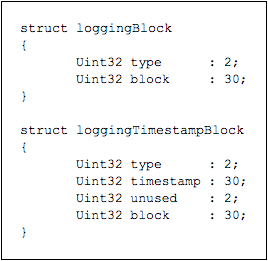
\includegraphics[width=3in]
  {code.png}}
  \caption{Example Logging Data Structures}
\end{figure}

\subsection{Drive Optimization}

A genetic algorithm ~\cite{GeneticAlgorithm, GAlib} is used to optimize the drive by intelligently reorganizing blocks and redefining precache groups on a periodic basis.  The process begins with an initial population of randomly generated organisms.  Each organism is represented by a logical to physical block mapping and the boundaries of the precache groups.  The fitness of each organism is calculated based on the efficiency with which the accesses in the logs would have been able to be performed given the organism's block mapping and precache groups.  Performance on older logs contributes less to fitness than performance on newer logs and the similarity of an organism to the current block organization and the logical block organization are also included in the fitness measure.  The most fit organisms are mated with a small probability of mutation to produce the next generation of organisms.  In the mating process the traits being expressed are precache groups.  Each offspring will have some combination of the precache groups of its parents.  In order to ensure that an offspring maps each logical block to one and only one physical block when a precache group is added from one parent all of the physical blocks in that group are removed from the precache groups of the other parent.  Removing these blocks will result in precache groups that become smaller over time.  In order to counteract this if the size of a precache group falls below a specified threshold that group is merged with the group that precedes it.  If the size of a precache group exceeds a specified threshold that group is split into smaller groups.  An example of the combination of two parents to form an offspring is shown below:

\begin{figure}[htb]
  \center{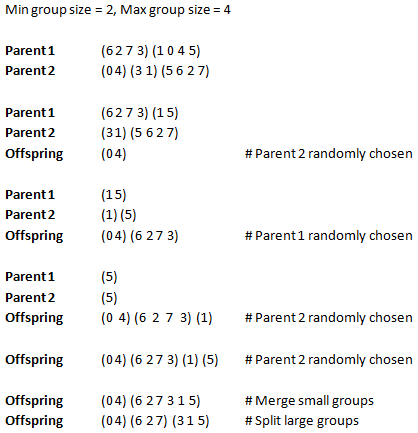
\includegraphics[width=3.5in]
  {ga-combination.png}}
  \caption{Genetic Algorithm Combination}
\end{figure}

The fitness of each generation is calculated and the organisms are mated to produce the next generation until a specified amount of time has elapsed or the fitness of the most fit individual does not improve for a specified number of generations.  The physical blocks are then reorganized to reflect the ordering specified by the mapping of the most fit organism and the precache boundaries are replaced with those of the most fit organism.

\section{Current Status}

The design phase of the project is complete and the implementation phase is currently in progress.  We have a functional implementation of a memory based Linux block device driver.  We have also completed implementation of a genetic algorithm for drive optimization.  Implementation of read/write of blocks on a raw partition and access logging is in progress.  Due to the complexity inherent in kernel mode programming the implementation phase of this project is progressing more slowly than was originally anticipated.  We are attempting to mitigate this issue by switching to an architecture which allows us to move much of the functionality to user space.  Our original schedule was also based on the optimistic assumption that we would be able to find or modify an existing machine learning algorithm implementation to meet our needs.  This did not happen and we required additional time to implement the algorithm.  The implication of these delays is that we will have less, although still sufficient, time to test the performance of the system.

\section{Implementation Plan}

\begin{description}
\item[4/01]
\end{description}
\begin{itemize}
\item Midterm report
\end{itemize}

\begin{description}
\item[4/01 - 4/04]
\end{description}
\begin{itemize}
\item Modification of Linux block device to issue requests to a user space daemon
\item Implementation of access logging
\end{itemize}

\begin{description}
\item[4/05 - 4/11]
\end{description}
\begin{itemize}
\item Modification of Linux block device to issue requests to a user space daemon
\item Implementation of access logging
\item Implementation of read/write of blocks on a raw partition
\item Implementation of intelligent precaching
\item Implementation of intelligent block reorganization
\end{itemize}

\begin{description}
\item[4/012 - 4/18]
\end{description}
\begin{itemize}
\item Definition of test workloads
\item Execution of test workloads
\end{itemize}

\begin{description}
\item[4/05 - 4/11]
\end{description}
\begin{itemize}
\item Execution of test workloads
\end{itemize}

\begin{description}
\item[4/24]
\end{description}
\begin{itemize}
\item Project presentation
\end{itemize}

\begin{description}
\item[4/24 - 5/10]
\end{description}
\begin{itemize}
\item Final performance evaluation
\end{itemize}

\begin{description}
\item[5/11]
\end{description}
\begin{itemize}
\item Final report and presentation 
\end{itemize}

\section{Evaluation}

 Due to our troubles with kernel programming, we have not been able to run any experiments yet and therefore do not have any numbers to share yet.
 
 \subsection{Experiments}
  As the implementation of our algorithm focuses on improving read access times, we will focus our attention on tasks that involve a large amount of disk reads.  Our path for evaluation will be to run different I/O intensive tasks with and without our changes.  We will measure the amount of disk block reads, the order in which the blocks are read, and the general amount of time to perform the task.  We will use the order of the block reads to determine if and how we might be able to improve our algorithms.  Measurements will be taken during our tests using a simple stopwatch and potentially a TBD OS-level performance-monitoring software.
  
In doing our measurements, we will be sure that the OS cache doesn't introduce too many variables in our measurements.  They best way to do this will be to make sure we are working with a clean cache in order to accurately measure our performance.  Using VMware to run Linux will be good for this since we can take snapshots and load those up quickly and reliably.
Some of the different types of I/O intensive tasks that we are currently considering include database usage, video and audio encoding/decoding, video and audio playback, software development activities (compilation, linking, loading of IDEs, etc.), and general computer usage (web browsing, email checking, word processing, etc). 

 \subsection{Results to be expected}
 Based on the use of the genetic algorithm, we expect that our project should speed up the results of our runs over time.  The main number that we will be measuring is the time it takes to perform activities, but the number of consecutive blocks that are read off of the hard drive will also be important (especially for cases where the hard drive isn't the bottleneck).

We expect our final project demo to perform better for some tasks, and perform as well or maybe worse for other tasks.  Based on other research papers that we have read, this seems to be the norm.  As long as we can show more of an improvement than deterioration, then we believe our project should be a success.  Also, if our approach is only good for specific activities (i.e., database accesses), then we could change the scope of our project from being a general purpose program to a specialized program that could be used specifically for those activities.

We have concerns that overhead of our system may severely worsen the results of our project.  We don't want accesses to take too long and we don't want there to be a lot of data stored per block.  Many processes are CPU intensive, and our program might slow down the CPU a little more.  With the rate CPU speed increases versus disk speed, it is probably better though for the CPU to take a hit.  One thing, that may be hard in achieving favorable results, is balancing the benefits that you get with the amount of information that you want to store.

We don't intend to have any improvements in write performance.  The knowledge of how blocks of data are read off of the hard drive, however, may provide potential side benefits to future work trying to improve write performance.

\section{Related Work}
While disk caching is not a particularly new idea, it is still an important area of study in computing systems as disk access times continue to be outpaced by other technological advances ~\cite{MultiplePrefetch}.  As disk access times have stagnated, though, disk capacity has grown dramatically.  The dynamics of this tradeoff has led systems to exploit caching where possible.  Some of the ideas that are being explored in our own research have also been studied in the past by other related work, so that is why the primary focus of our effort has been on the application of machine learning algorithms in this domain.  Some related work included elements of machine learning in their basic caching and rearrangement algorithms, but these were not the main focus of their study.  The following work helped us direct and adapt our own study as we learned the techniques that had been used in the past.  Overall, it was surprising that much of this prior work was performed at least a decade ago, but despite the notion that disk caching was already a solved problem, we felt that there might still be room for improvement through use of more advanced algorithms.

In work by Grimsrud, Archibald, and Nelson ~\cite{MultiplePrefetch}, we studied how they had developed new approaches of using prefetching schemes to improve disk access performance.  Their scheme was designed to be more sophisticated than simple precaching of disk blocks ahead of those currently being read.  Instead, they developed prefetching that could adapt its efforts based on what it had seen in prior disk accesses.  Its role in detecting useful disk access patterns would in turn result in more efficient prefetching decisions for future disk accesses.  Finding that the authors based their testing methodology on trace-driven simulation gave us confidence in our choice of using DiskSim ~\cite{DiskSimManual}.

The main avenues for disk access optimization in our design are through effective prefetching and block rearrangement.  Therefore, it was very important for us to understand how existing prefetching strategies work, as well as how to avoid any of the pitfalls that previous researchers had faced.  A key point made by Grimsrud, et al., is that one must be diligent about ensuring reliable accuracy when prefetching, for a poorly design prefetching scheme can decrease disk performace due to pollution of the cache and unexpected congestion.  Another key concept from this paper comes from their use of an adaptive table which stores the most likely successive disk accesses after a particular block has been accessed.  This concept can be much more effective than simply prefetching blocks sequentially beyond the particular block.

Our approach to implementing and testing our algorithmic improvements to disk drive read accesses was to develop a disk block device driver for Linux.  By using a Linux block device driver, the physical drive and partitions were abstracted and we could control a layer below the filesystem.  In controlling this layer, we decided that using a logical to physical block mapping would give us precise, low-level control over which blocks would be accessed whenever the filesystem presented a request.  At the same time, this mapping would give us the ability to perform block rearrangement virtually without ever having to physically move disk blocks if so desired ~\cite{Loge}.  We researched work on the Logical Disk (LD) by de Jonge, Kaashoek, and Hsieh ~\cite{LogicalDisk} to help us understand what concepts were found to be important in developing a system with this type of indirection mapping.  The Logical Disk was shown to deliver a useful abstraction layer without a detrimental effect on efficiency.  This added layer does not come completely free, as there is added storage overhead required in order to maintain the logical to physical block mapping.

Finally, we studied the work of Akyurek and Salem on Adaptive Block Rearrangement ~\cite{AdaptiveBlock}.  Block rearrangement will be one of the most important functions of our technique, as it is the efficient placement of blocks that will in turn allow for reduced disk access times when disk requests are made and precaching is in use.  In Akyurek and Salem's work, their adaptive algorithm requires no prior knowledge of the type of information it will encounter in order to perform effectively, and with our use of a genetic algorithm, our method will not require prior knowledge to perform either.  Our technique, however, does differ from Akyurek and Salem's in how it adapts to the incoming information stream.  While their algorithm merely uses frequencies to estimate which block will most likely follow a given block, we use a more sophisticated, genetic algorithm that learns as it continues to process new disk requests.  This difference marks our primary goal of determining if advanced machine learning algorithms can improve disk drive read access performance.

{\footnotesize \bibliographystyle{acm}
\bibliography{./midterm}}

\end{document}







